\documentclass[12pt,a4paper]{article}
\usepackage[UTF8]{ctex}     %先引入ctex
\usepackage[utf8]{inputenc} %再引入inputenc
\usepackage{graphicx}
\usepackage{geometry}
\usepackage{xcolor}
% \usepackage{lazylatex}
\usepackage{amsmath}
\usepackage{enumerate}
\usepackage{caption}
\usepackage{listings}
\captionsetup[lstlisting]{labelfont=bf,justification=justified}

\usepackage{tikz}

\graphicspath{{img/}}
% 边距
\geometry{left=2.0cm,right=2.0cm,top=2.0cm,bottom=3.0cm}
% 大题
\newenvironment{problems}{\begin{list}{}{\renewcommand{\makelabel}[1]{\textbf{##1}\hfil}}}{\end{list}}
% 小题
\newenvironment{steps}{\begin{list}{}{\renewcommand{\makelabel}[1]{##1.\hfil}}}{\end{list}}
% 答
\providecommand{\ans}{\textbf{答}:~}
% 解
\providecommand{\sol}{\textbf{解}.~}

\usepackage[colorlinks,linkcolor=blue]{hyperref}
\usepackage{bookmark}
\providecommand{\code}[2]{\lstinputlisting[language=#2,caption=\href{run:#1}{\ttfamily #1}]{#1}}
\providecommand{\img}[1]{\includegraphics[width=0.88\textwidth]{#1}}

% listings
\definecolor{grey}{rgb}{0.8,0.8,0.8}
\definecolor{darkgreen}{rgb}{0,0.3,0}
\definecolor{darkblue}{rgb}{0,0,0.3}
\lstset{%
    % numbers=left, %行号
    % numberstyle=\tiny\color{grey},
    showstringspaces=false,
    showspaces=false,%
    tabsize=4,%
    frame=shadowbox,%
    basicstyle={\ttfamily\scriptsize},%
    keywordstyle=\color{blue!80!black}\bfseries,%
    identifierstyle=,%
    commentstyle=\color{green!50!blue}\itshape,%
    stringstyle=\color{green!50!black},%
    rulesepcolor=\color{gray!20!white},
    breaklines,
    columns=flexible,
    extendedchars=false,
    %mathescape=true,
}

\begin{document}
\title{\normalsize \underline{操作系统(D)}\\\LARGE 项目 2}
\author{李子龙 518070910095}
\date{\today}
\maketitle

\begin{problems}
    \item[一] \textbf{Unix 外壳程序}
    \begin{steps}
        
        \item[1] 在子进程中执行命令
        
        \img{ps.png}

        同时执行命令:

        \img{psc.png}

        当输入 \verb"exit" 时,会退出外壳程序:

        \img{exit.png}

        可以看到外壳主进程在子进程尚未打印完成前就已经开始等待用户输入了,也就是两个进程同时进行。

        该部分需要获取用户输入,这里采用了 \texttt{fgets} 函数获取用户的整行输入。
        \begin{lstlisting}[language=c]
            fgets(rline, MAX_LINE, stdin);
        \end{lstlisting}
        第二参数用于说明最大读入字符数,将会限定最大的范围防止越界。该函数也支援存储换行符 \verb"\n"。

        在遍历输入字符时,如果遇到 \verb"&" 字符,将会对 \verb"should_wait" 标志置为 0,
        \begin{lstlisting}[language=c]
            case '&':
                should_wait = 0;
        \end{lstlisting}
        在之后的子进程创建函数中将会根据这个标志判定是否等待:
        \begin{lstlisting}[language=c]
            pid_t pid;
            pid = fork();

            if (pid < 0) fprintf(stderr, "Fork Failed"); 
            else if (pid == 0) return execvp(args[0],args);
            else if (should_wait) wait(NULL);
        \end{lstlisting}

        对于 \verb"args" 数组的存储,将会将每个字符串数组的起始位置指向 \verb"rline" 用户输入数组的对应位置(该过程通过判定前一个字符是否是空格实现),以实现参数存储
        \begin{lstlisting}[language=c]
            default:
                if (prev == ' ') args[argc++] = rptr;
                prev = *rptr;
                break;
        \end{lstlisting}
        
        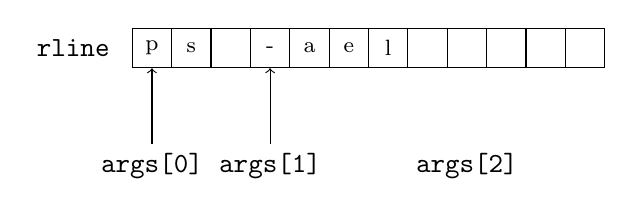
\begin{tikzpicture}
\tikzstyle{box} = [minimum width=0.5cm, minimum height=0.5cm, draw, font=\footnotesize];

\foreach \x/\y in {1/p,2/s,3/,4/-,5/a,6/e,7/l,8/,9/,10/,11/,12/}
	\node[box] (n-\x) at (\x*0.5,0) {\y};

\node at (-0.5,0) {\texttt{rline}};
\node (t-0) at (0.5,-1.5) {\verb"args[0]"};
\draw[->] (t-0) edge (n-1);
\node (t-1) at (2,-1.5) {\verb"args[1]"};
\draw[->] (t-1) edge (n-4);
\node at (4.5,-1.5) {\verb"args[2]"};
\end{tikzpicture}


        当遇到空格、换行、\verb"&"符号时,都会被替换为 \verb"\0",从而限制每一个字符串数组的终止位置
        \begin{lstlisting}[language=c]
            case '&':
                should_wait = 0;
            case '\n':
                flag = 1;
            case ' ':
                prev = *rptr;
                *rptr = '\0';
                break;
        \end{lstlisting}

        最后一个参数根据规定,必须被赋值为空指针
        \begin{lstlisting}[language=c]
            args[argc] = NULL;
        \end{lstlisting}

        退出的判定是通过 \verb"strcmp" 函数实现的
        \begin{lstlisting}[language=c]
            should_run = strcmp(args[0],"exit");
        \end{lstlisting}

        \item[2] 历史记录存储
        
        当输入 \verb"!!" 时将会回显并运行上一条指令

        \img{history.png}

        当没有上一条指令时,将会返回提示

        \img{nohist.png}

        这一部分需要将上一条指令存储在 \texttt{buf} 中,开始时置为空
        \begin{lstlisting}[language=c]
            char buf[MAX_LINE] = "\0";
        \end{lstlisting}

        当连续输入两个 \verb"!" 时,将会首先检查 \verb"buf[0]" 是否是空字符,否则将通过 \verb"memcpy" 将缓存复制到当前的阅读行数组中,注意这里不能使用 \verb"strcpy",因为其的复制到 \verb"\0" 就会立刻停止,导致后面的部分没有被有效复制。循环条件也增加了 \verb"flag" 判定。
        \begin{lstlisting}[language=c]
            for(char* rptr = rline; rptr < rline + MAX_LINE && !flag; ++rptr){
                //...
                case '!':
                    if (prev=='!' && argc == 0){
                        if(!buf[0]){
                            fprintf(stdout, "%s\n", "No commands in history.");
                            flag = -1;
                        } else {
                            memcpy(rline, buf, MAX_LINE*sizeof(char));
                            fprintf(stdout, "%s\n", rline);
                            flag = 2;
                        }
                    }
                    prev = *rptr;
                    break;
                //...
        \end{lstlisting}

        如果是正常指令,就会将当前指令复制到缓冲区中去。如果不是正常指令,将不会执行任何指令。
        \begin{lstlisting}[language=c]
            switch(flag){
                case 1:
                    args[argc] = NULL;
                case 2:
                    if (!args[0]) break;
                    memcpy(buf, rline, MAX_LINE*sizeof(char));
                    should_run = strcmp(args[0],"exit");
                    
                    // run the fork part
            }
        \end{lstlisting}

        \item[3] 重定向输入输出
        
        
        \item[4] 
        使用下面的 Makefile 编译:
        \code{src/Makefile}{}

    \end{steps} 
    \item[二]  

\end{problems}


\end{document}
